\chapter{Linear functions}
\label{ch:linear}

\chapquote{A curve does not exist in its full power until contrasted with a straight line.}{Robert Henri, American painter}

So far we have learned quite a bit about the family of linear functions. From our work with sequences we learned how to tell if a sequence was arithmetic. We can write recursive rules for arithmetic sequences, and we can change those recursive rules into into explicit formulas.

We turned arithmetic sequences into tables of data, and when we graphed some linear functions, we saw that all were straight lines. We saw a preview of how different transformations might change the way its graph looks.

Most recently we learned about a specific type of linear function, the direct variation. In this chapter we will bring together all of the pieces we have learned previously into a single coherent, and very important, concept.

% % % % % % % % % % % % % % % % % % % % % % % % % % % % % % % % % % % % % % % %
\section{Rate of change and slope}
\label{sec:rateofchange}

%\begin{boxexplore}[Extended exploration: Calculating speed]
%\addtodoitem{Click here to visit the extended exploration: Calculating Speed}
%\end{boxexplore}
\addtodoitem{Link to extended exploration: Calculating speed}

\begin{boxexplore}[CCC]
Bob enrolls at Cheeseville Community College, and the admissions counselor there gives him the following table estimating the cost to attend. The total cost of a semester at CCC is made up of two expenses: (a) the fixed fees, which are the same for every student every semester (technology fee, printing allowance, and so on), and (b) the tuition rate, which varies per credit hour.

Most courses at CCC are either 3 or 4 credit hours per semester. The table summarizes several combinations of 3- and 4-hour courses.

\kverse{Bob enrolls at Cheeseville Community College}

\begin{center}
\begin{tabularx}{0.75\linewidth}{|c|*{5}{>{\centering\arraybackslash}X}|}
\hline
No. Credit Hours & 3 & 4 & 6 & 7 & 10 \\\hline
Cost (dollars) & 501 & 654 & 960 & 1113 & 1572\\\hline
\end{tabularx}
\end{center}

What can you learn from the table? How much is tuition per credit hour? How much does CCC estimate Bob will pay in fees?
\end{boxexplore} %% End of startup exploration

\subsection{Unit rates in data}

Since we're fresh from a discussion of proportional reasoning, perhaps our first guess might be that this is a direct variation. Unfortunately, a quick check of the ratios $\frac{y}{x}$ shoots that idea down: \[\frac{501}{3} = 167 \qquad\text{but}\qquad \frac{654}{4} = 163.5\]
Maybe we have an arithmetic sequence? If so, then the terms of the ``cost'' sequence will have a constant difference. But, if we take the differences between neighboring terms, we have different values: \[654 - 501 = 153 \qquad\text{but}\qquad 906-654 = 306\]
But, hang on. Look at the corresponding ``number of credit hours''. These numbers don't increase by the same amount at every step, like they did for our arithmetic sequences. There's a jump from 4 to 6. We're going to have to be a bit more clever to account for this!

Notice that when ``credit hours'' increases by 1, ``cost'' increases by \$153. And then, when ``credit hours'' increases by 2, ``cost'' increases by \$306 -- the increase in both values has doubled! This even works at the end of the table: When the number of hours jumps by 3 and the cost jumps by \$459, the rate ``\$dollars per 1 credit hour'' says the same:
\[\frac{153}{1} = \frac{306}{2} = \frac{459}{3} = \frac{\text{change in the total cost}}{\text{change in the number of hours}}\]
So, even though the table skips over some numbers, the \textit{change} in the cost still corresponds to the \textit{change} in the number of hours. So, the tuition rate at CCC must be \$153 per credit hour.


%%% The amount Bob will pay in fees is the amount that stays fixed regardless of how many credit hours Bob takes. Theoretically, even if Bob took ``0 hours'', he would still pay the fees. How much would Bob pay to take 0 hours? We simply back up one hour in the table (we take away \$153 from the cost of taking 1 hour) and discover that Bob will pay \$42 in fees.

\begin{boxex}
Does the data in the table below represent someone moving at a constant speed? If so, what is the speed?

\begin{center}
\begin{tabular}{|C{2cm}|C{2cm}|}
\hline
\text{Time (sec)} & \text{Distance (m)}\\\hline
5 & 17.5\\
12 & 42.0\\
31 & 108.5\\\hline
\end{tabular}
\end{center}

\exsoln\ Comparing the first two data points, we see that the change in distance is $42.0 - 17.5 = 24.5$ meters, and that this occurs over $12-5=7$ seconds. This ratio ``24.5 meters per 7 seconds'' corresponds to the unit rate ``3.5 meters per second''.

Comparing the second pair of data points, we see that a change in distance of $108.5-42.0 = 66.5$ meters happens over $31-12 = 19$ seconds. The ratio ``66.5 meters per 19 seconds'' corresponds to the unit rate ``3.5 meters per second''.

So, yes, this table does represent movement at a constant speed of 3.5 meters per second.
\end{boxex}

%Movement at a constant speed -- a constant change in distance over a certain unit of time -- is what generated a straight line. So, if I can find speed from a table, I can check if it is constant, and, without graphing, determine if the data is linear.

\subsection{Rate of change}

We want to be able to tell if \textit{any} data set is linear. The examples of speed and hourly tuition begin to suggest a general approach. We are seeking a constant \gls{rate of change}.

\begin{boxdef}[Rate of change]
Rate of change is a measurement of how quickly the dependent variable changes relative to a one-unit change in the independent variable.
\end{boxdef}

To compute the rate of change of $y$ with respect to $x$, we want to ``unitize'' a change in $y$ (the dependent variable) with respect to the corresponding change in $x$ (the independent variable).

To write this out using mathematical notation, we use an abbreviation for the idea of ``change'': the Greek letter delta, $\Delta$. This makes the definition of rate of change look like the following:
\[R.O.C. = \frac{\Delta \text{ dependent variable}}{\Delta \text{ independent variable}} = \frac{\Delta y}{\Delta x}\]
The symbol ``$\Delta y$'' is pronounced ``delta $y$'' or ``change in $y$''. We sometimes say that rate of change is ``delta $y$ over delta $x$''.

%Note again that this is not ``divide $y$ by $x$'', but ``divide (change between two $y$ values) by (corresponding change between tow $x$ value)''.
%%% ADD WHY THAT WORKS FOR D.V.

Speed is an example of a rate of change. It is a measurement of how distance changes relative to a one-unit change in time: meters per (one) second. Bob's tuition at Cheeseville Community College is another example that measures how his total expense changes relative to a unit-change in the number of credit hours he takes: dollars per (one) hour.


% % % % % % % % % % % % % % % % % % % % % % % % % % % % % % % % % % % % % % % % 
\subsection{Slope}

Rate of change is a very important concept in mathematics and it is a general term that doesn't just apply to straight lines. Different types of functions have different patterns emerge in their rates of change. The study of rate of change led to the development of calculus!

But, the rate of change of a straight line is special: it's always the same. When it comes to linear relationships, the key is knowing that the \textit{rate of change for linear data is constant}. We have a special term for the rate of change in a linear relationship.

\begin{boxdef}[Slope]
\Gls{slope} is a measurement of the steepness of a line.
\end{boxdef}

For a line, slope and rate of change are describing the same thing. We don't really talk about the ``slope'' of a curve (like the graph of an exponential and quadratic functions), since the steepness changes, as we saw in \cref{sec:interpgraphs}.

In mathematical notation, the letter most often used to abbreviate slope is $m$.\footnote{``Why $m$?'' we bet you're wondering. Many people have looked into this question, digging back through mathematical writing to try and learn where this abbreviation comes from. It seems that the earliest recorded use of $m$ for slope was in 1757 by Italian mathematician Vincenzo Riccati. But his work includes no explanation of \textit{why} the letter $m$ was used.} So, we can update our notation from earlier:
\[m = \frac{\Delta y}{\Delta x}\]

\subsubsection{Slope from data}

As we have seen in the earlier examples, finding slope from a data table is rather easy. We find the change between two $y$-values and find the change between the corresponding $x$-values. When we unitize this ratio -- in other words, when we divide $\Delta y$ by $\Delta x$ -- we've got slope. Woot!

This works even if the data is not given in table form. You may have heard the old saying, ``The shortest distance between two points is a straight line.'' Well\ldots\ what's the slope of that line?

\begin{boxex}
Find the slope of the line connecting the points $(11, 4)$ and $(16, 29)$.

\exsoln\ The change in the $y$-values is $\Delta y = 29-4 = 25$, and the change in the $x$-values is $\Delta x = 16-11=5$. So, the slope of the line between these two points is \[m = \frac{\Delta y}{\Delta x} = \frac{25}{5} = 5.\]
So, the line connecting the points $(11, 4)$ and $(16, 29)$ has a slope of 5.
\end{boxex}

\subsubsection{Slope from a graph: The slope triangle}

Suppose we're given the graph of a line and asked to find the slope. We could create a data table using points on the line and find the slope from that data. Or, we could inspect the graph directly using a \textit{slope triangle}. A slope triangle is a right triangle that connects two points with a single vertical move and a single horizontal move.

Here is the graph of a line with some points marked. To find the slope of the line, we draw a slope triangle.

\resizeplot{-5}{-4}{7}{8}

\begin{center}
\begin{minipage}{0.49\textwidth}
	\centering
	\begin{tikzpicture}
		\begin{axis}[
			standard,
			width=\linewidth,
			height=\linewidth,
			minor xtick={-5,...,7},
			minor ytick={-4,...,8},
		]
			\addplot[algcurve, violet, domain=-5:7] (\x,0.667*\x+3);
%			\draw[violet] (axis cs:4,-3,0) node[right]{\large$y=\frac{1}{3}x-4$};
			\addplot[algpoints, violet] coordinates {(-3,1)(0,3)(3,5)(6,7)};
		\end{axis}
	\end{tikzpicture}
%	\begin{tikzpicture}[scale=0.5]
%		%% grid setup
%		\draw[very thin, color=gray!25] (-5,-4) grid (7, 8);
%		\draw[<->,thick] (-5,0) -- (7,0); % node[right]{$x$-axis};
%		\draw[<->,thick] (0,-4) -- (0,8); % node[above]{$y$-axis};
%		\foreach \x in {-5,...,7} \draw (\x,0.05) -- (\x,-0.05) node[below] {\footnotesize\x};
%		\foreach \y in {-4,...,8} \draw (-0.05,\y) -- (0.05,\y) node[left] {\footnotesize\y};
%		%% graph
%		\draw[<->, very thick, violet, domain=-5:7] plot (\x,0.667*\x+3);
%		%% points (top layer)
%		\draw[violet] plot[only marks, mark=*, mark size=4] coordinates {(-3,1)(0,3)(3,5)(6,7)};
%	\end{tikzpicture}
\end{minipage}
%
\begin{minipage}{0.49\textwidth}
	\centering
	\begin{tikzpicture}
		\begin{axis}[
			standard,
			width=\linewidth,
			height=\linewidth,
			minor xtick={-5,...,7},
			minor ytick={-4,...,8},
		]
			\addplot[algcurve, violet, domain=-5:7] (\x,0.667*\x+3);
%			\draw[violet] (axis cs:4,-3,0) node[right]{\large$y=\frac{1}{3}x-4$};
			\addplot[algpoints, violet] coordinates {(-3,1)(0,3)(3,5)(6,7)};
			%% slope triangle
			\draw[->, very thick, red] (axis cs: 3,5) -- (axis cs: 3,7);
			\draw[red] (axis cs: 3,6) node[left] {+2};
			\draw[->, very thick, blue] (axis cs: 3,7) -- (axis cs: 6,7);
			\draw[blue] (axis cs: 4.5,7) node[above] {+3};
		\end{axis}
	\end{tikzpicture}
%
%	\begin{tikzpicture}[scale=0.5]
%		%% grid setup
%		\draw[very thin, color=gray!25] (-5,-4) grid (7, 8);
%		\draw[<->,thick] (-5,0) -- (7,0); % node[right]{$x$-axis};
%		\draw[<->,thick] (0,-4) -- (0,8); % node[above]{$y$-axis};
%		\foreach \x in {-5,...,7} \draw (\x,0.05) -- (\x,-0.05) node[below] {\footnotesize\x};
%		\foreach \y in {-4,...,8} \draw (-0.05,\y) -- (0.05,\y) node[left] {\footnotesize\y};
%		%% graph
%		\draw[<->, very thick, violet, domain=-5:7] plot (\x,0.667*\x+3);
%		\draw[violet] plot[only marks, mark=*, mark size=4] coordinates {(-3,1)(0,3)(3,5)(6,7)};
%		%% slope triangle
%		\draw[->, very thick, red] (3,5) -- (3,7);
%		\draw[red] (3,6) node[left] {\bfseries+2};
%		\draw[->, very thick, blue] (3,7) -- (6,7);
%		\draw[blue] (4.5,7) node[above] {\bfseries+3};
%	\end{tikzpicture}
\end{minipage}
\end{center}
the red arrow shows the vertical change. It starts at 5 and goes to 7, a vertical distance of $7-5=2$ units. The blue arrow shows the horizontal change. It starts at 3 and goes to 6, a horizontal change of $6-3=3$ units. Now we can calculate slope \[m = \frac{\text{vertical change}}{\text{horizontal change}} = \frac{2}{3}.\] Since the rate of change is constant for a straight line, it doesn't matter which two points we choose, or which point we choose as the starting place. Each of the slope triangles below can be used to compute slope of this line!

\begin{center}
\begin{minipage}{0.32\textwidth}
	\centering
	\begin{tikzpicture}
		\begin{axis}[
			standard,
			width=\linewidth,
			height=\linewidth,
			minor xtick={-5,...,7},
			minor ytick={-4,...,8},
		]
			\addplot[algcurve, violet, domain=-5:7] (\x,0.667*\x+3);
%			\draw[violet] (axis cs:4,-3,0) node[right]{\large$y=\frac{1}{3}x-4$};
			\addplot[algpoints, violet] coordinates {(-3,1)(0,3)(3,5)(6,7)};
			%% slope triangle
			\draw[->, very thick, red] (axis cs: -3,1) -- (axis cs: -3,7);
			\draw[red] (axis cs: -3,4) node[left] {\bfseries+6};
			\draw[->, very thick, blue] (axis cs: -3,7) -- (axis cs: 6,7);
			\draw[blue] (axis cs: 2.5,7) node[above] {\bfseries+9};
		\end{axis}
	\end{tikzpicture}
%
%	\begin{tikzpicture}[scale=0.4]
%		%% grid setup
%		\draw[very thin, color=gray!25] (-5,-4) grid (7, 8);
%		\draw[<->,thick] (-5,0) -- (7,0); % node[right]{$x$-axis};
%		\draw[<->,thick] (0,-4) -- (0,8); % node[above]{$y$-axis};
%		\foreach \x in {-4,-2,2,4,6} \draw (\x,0.05) -- (\x,-0.05) node[below] {\footnotesize\x};
%		\foreach \y in {-4,-2,...,8} \draw (-0.05,\y) -- (0.05,\y) node[left] {\footnotesize\y};
%		%% graph
%		\draw[<->, very thick, violet, domain=-5:7] plot (\x,0.667*\x+3);
%		\draw[violet] plot[only marks, mark=*, mark size=6] coordinates {(-3,1)(0,3)(3,5)(6,7)};
%		%% slope triangle
%		\draw[->, very thick, red] (-3,1) -- (-3,7);
%		\draw[red] (-3,4) node[left] {\bfseries+6};
%		\draw[->, very thick, blue] (-3,7) -- (6,7);
%		\draw[blue] (1.5,7) node[above] {\bfseries+9};
%	\end{tikzpicture}
\end{minipage}
%
\begin{minipage}{0.32\textwidth}
	\centering
	\begin{tikzpicture}
		\begin{axis}[
			standard,
			width=\linewidth,
			height=\linewidth,
			minor xtick={-5,...,7},
			minor ytick={-4,...,8},
		]
			\addplot[algcurve, violet, domain=-5:7] (\x,0.667*\x+3);
%			\draw[violet] (axis cs:4,-3,0) node[right]{\large$y=\frac{1}{3}x-4$};
			\addplot[algpoints, violet] coordinates {(-3,1)(0,3)(3,5)(6,7)};
			%% slope triangle
			\draw[->, very thick, red] (axis cs: -3,1) -- (axis cs: -3,5);
			\draw[red] (axis cs: -3,3) node[left] {\bfseries+4};
			\draw[->, very thick, blue] (axis cs: -3,5) -- (axis cs: 3,5);
			\draw[blue] (axis cs: 1,5) node[above] {\bfseries+6};
		\end{axis}
	\end{tikzpicture}
%
%	\begin{tikzpicture}[scale=0.4]
%		%% grid setup
%		\draw[very thin, color=gray!25] (-5,-4) grid (7, 8);
%		\draw[<->,thick] (-5,0) -- (7,0); % node[right]{$x$-axis};
%		\draw[<->,thick] (0,-4) -- (0,8); % node[above]{$y$-axis};
%		\foreach \x in {-4,-2,2,4,6} \draw (\x,0.05) -- (\x,-0.05) node[below] {\footnotesize\x};
%		\foreach \y in {-4,-2,...,8} \draw (-0.05,\y) -- (0.05,\y) node[left] {\footnotesize\y};
%		%% graph
%		\draw[<->, very thick, violet, domain=-5:7] plot (\x,0.667*\x+3);
%		\draw[violet] plot[only marks, mark=*, mark size=6] coordinates {(-3,1)(0,3)(3,5)(6,7)};
%		%% slope triangle
%		\draw[->, very thick, red] (-3,1) -- (-3,5);
%		\draw[red] (-3,3) node[left] {\bfseries+4};
%		\draw[->, very thick, blue] (-3,5) -- (3,5);
%		\draw[blue] (1,5) node[above] {\bfseries+6};
%	\end{tikzpicture}
\end{minipage}
%
\begin{minipage}{0.32\textwidth}
	\centering
	\begin{tikzpicture}
		\begin{axis}[
			standard,
			width=\linewidth,
			height=\linewidth,
			minor xtick={-5,...,7},
			minor ytick={-4,...,8},
		]
			\addplot[algcurve, violet, domain=-5:7] (\x,0.667*\x+3);
%			\draw[violet] (axis cs:4,-3,0) node[right]{\large$y=\frac{1}{3}x-4$};
			\addplot[algpoints, violet] coordinates {(-3,1)(0,3)(3,5)(6,7)};
			%% slope triangle
			\draw[->, very thick, red] (axis cs: 3,5) -- (axis cs: 3,1);
			\draw[red] (axis cs: 3,3) node[right] {\bfseries--4};
			\draw[->, very thick, blue] (axis cs: 3,1) -- (axis cs: -3,1);
			\draw[blue] (axis cs: 1,1) node[below] {\bfseries--6};
		\end{axis}
	\end{tikzpicture}
%
%	\begin{tikzpicture}[scale=0.4]
%		%% grid setup
%		\draw[very thin, color=gray!25] (-5,-4) grid (7, 8);
%		\draw[<->,thick] (-5,0) -- (7,0); % node[right]{$x$-axis};
%		\draw[<->,thick] (0,-4) -- (0,8); % node[above]{$y$-axis};
%		\foreach \x in {-4,-2,2,4,6} \draw (\x,0.05) -- (\x,-0.05) node[below] {\footnotesize\x};
%		\foreach \y in {-4,-2,...,8} \draw (-0.05,\y) -- (0.05,\y) node[left] {\footnotesize\y};
%		%% graph
%		\draw[<->, very thick, violet, domain=-5:7] plot (\x,0.667*\x+3);
%		\draw[violet] plot[only marks, mark=*, mark size=6] coordinates {(-3,1)(0,3)(3,5)(6,7)};
%		%% slope triangle
%		\draw[->, very thick, red] (3,5) -- (3,1);
%		\draw[red] (3,3) node[right] {\bfseries--4};
%		\draw[->, very thick, blue] (3,1) -- (-3,1);
%		\draw[blue] (1,1) node[below] {\bfseries--6};
%	\end{tikzpicture}
\end{minipage}
\end{center}

Again, we don't have to use a slope triangle. We can just convert at least two of the points on the graph into a table and then use the techniques for finding slope from a data set.

There are two commonly mixed up things about slope. First: reciprocalizing the ratio. Remember it's change in $y$ over change in $x$, not the other way around.

Second, folks sometimes have problems with sign. A rule of thumb: if the data has a positive correlation, the slope is positive. If the data has a negative correlation, the slope is negative. It's a good habit always to double-check the sign of a slope to verify that it makes sense in context.

\begin{boxex}
Find the slope of the line depicted in the following graph.

\begin{center}
	\resizeplot{-10}{-20}{10}{20}
	\begin{tikzpicture}
		\begin{axis}[
			standard,
%			width=\linewidth,
%			height=\linewidth,
%			minor xtick={-5,...,7},
%			minor ytick={-4,...,8},
		]
			\addplot[algcurve, violet, domain=-6:10] (\x,-2.5*\x+5);
%			\draw[violet] (axis cs:4,-3,0) node[right]{\large$y=\frac{1}{3}x-4$};
			\addplot[algpoints, violet] coordinates {(-4,15)(6,-10)};
		\end{axis}
	\end{tikzpicture}
\end{center}
%\begin{center}
%	\begin{tikzpicture}[xscale=0.3, yscale=0.15]
%		%% grid setup
%		\draw[very thin, color=gray!25, xstep=2, ystep=5] (-10,-20) grid (10, 20);
%		\draw[<->,thick] (-10,0) -- (10,0); % node[right]{$x$-axis};
%		\draw[<->,thick] (0,-20) -- (0,20); % node[above]{$y$-axis};
%		\foreach \x in {-10,-8,...,10} \draw (\x,0.05) -- (\x,-0.05) node[below] {\footnotesize\x};
%		\foreach \y in {-20,-15,...,20} \draw (-0.05,\y) -- (0.05,\y) node[left] {\footnotesize\y};
%		%% graph
%		\draw[<->, very thick, violet, domain=-6:10] plot (\x,-2.5*\x+5);
%		%% points (top layer)
%		\fill[violet] (-4,15) circle[x radius=.3, y radius=.6];
%%		\fill[violet] (-2,10) circle[x radius=.3, y radius=.6];
%%		\fill[violet] (0,5) circle[x radius=.3, y radius=.6];
%%		\fill[violet] (2,0) circle[x radius=.3, y radius=.6];
%%		\fill[violet] (4,-5) circle[x radius=.3, y radius=.6];
%		\fill[violet] (6,-10) circle[x radius=.3, y radius=.6];
%%		\fill[violet] (8,-15) circle[x radius=.3, y radius=.6];
%	\end{tikzpicture}
%\end{center}

\exsoln\ This problem exhibits two key features: the slope of the line will be negative (since the line decreases as we move to the right), and we're going to have to be careful about the scale on the axes! We might see a vertical change of one ``tick mark'' on the axis, but note that one tick mark is a change of 5 units. Similarly, one tick on the $x$-axis is a change of two units.

If we start at the point on the left and move to the point on the right, we have a horizontal change of +10 units in the horizontal direction and $-25$ units in the vertical direction (a negative vertical change means moving downwards). So, the slope is \[m = \frac{-25}{10} = \frac{-5}{2} = -\frac{5}{2}\]
\end{boxex}

\subsection{Slope formula}

The process of computing slope is always basically the same, so we can derive a formula for slope. Study the picture below, showing a line through two ``generic points'' called $(x_1,y_2)$ and $(x_2,y_2)$.

\begin{center}
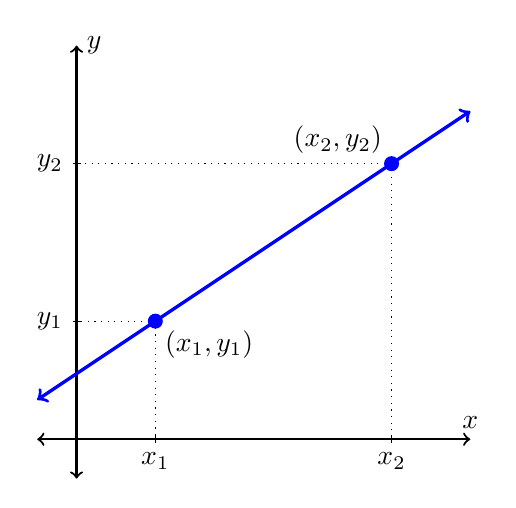
\begin{tikzpicture}[scale=0.5]
	%% grid setup
%	\draw[very thin, color=gray!25] (0,0) grid (10,10);
	\draw[<->,thick] (-1,0) -- (10,0) node[above] {$x$};
	\draw[<->,thick] (0,-1) -- (0,10) node[right] {$y$};
	%% line segment
	\draw[<->, very thick, blue] (-1,1) -- (10,8.333); % node[right] {$x$};
	\draw (2,3) node[below right] {$(x_1, y_1)$};
	\draw (8,7) node[above left] {$(x_2, y_2)$};
	%% horizontal labels
	\draw[dotted] (2,3) -- (2,0);
	\draw (2,0.1) -- (2,-0.1) node[below]{$x_1$};
	\draw[dotted] (8,7) -- (8,0);
	\draw (8,0.1) -- (8,-0.1) node[below]{$x_2$};
	%% vertical labels
	\draw[dotted] (2,3) -- (0,3);
	\draw (0.1,3) -- (-0.1,3) node[left]{$y_1$};
	\draw[dotted] (8,7) -- (0,7);
	\draw (0.1,7) -- (-0.1,7) node[left]{$y_2$};
	%% points
	\draw[blue] plot[only marks,mark=*,mark size=5] coordinates{(2,3)(8,7)};
\end{tikzpicture}
\end{center}

The vertical change between the two points is $y_2 - y_1$, and the horizontal change is $x_2 - x_1$. So we can compute the slope between these two points using our familiar formula \[m = \frac{\Delta y}{\Delta x} = \frac{y_2 - y_1}{x_2 - x_1}.\] The trickiest part about using this formula is being consistent about which point we call $(x_1, y_1)$ and which point we call $(x_2,y_2)$. It doesn't matter which point is which -- but we have to be consistent.

\begin{boxdef}[Tangent: Order of the points]
That last sentence says ``it doesn't matter which point is which.'' Why is that? Explain why it doesn't matter which point we call ``point 1'' and which we call ``point 2''. In other words, if we have two points called $(x_1, y_1)$ and $(x_2,y_2)$, explain why \[\frac{y_2 - y_1}{x_2 - x_1} = \frac{y_1 - y_2}{x_1 - x_2}.\] (Hint: Experiment with some numbers first, then try to extend your observations to the two ``generic'' points given.)
\end{boxdef}

\subsection{Horizontal and vertical lines}

If we think about how slope is calculated -- vertical change over horizontal change -- a horizontal line has \textit{no vertical change}, or a vertical change of zero. If we pick two points on a horizontal line and calculate slope, we would get 0 divided by some number, which always equals zero! So the slope of a horizontal line is always 0. This makes sense if we remember the slope is a measure of the steepness: a horizontal line is flat, and that means no ``steepness'' at all!

If we pick two points on a vertical line and try to calculate slope, we will get a horizontal change of 0. So we'll have some number divided by 0\ldots\ and that's off limits. We say that the slope of a vertical line is \textit{undefined}, since division by 0 is undefined.

\subsection{Using slope}

Before, when we were graphing a line we had to take some domain values, like the integers between $–3$ and $3$, plug them in to the equation, and plot every single point, one at a time. Now we have an alternative!

All we really need to graph a line is two points. If we have one point on the line and the \textit{slope}, we can find another point on the line.

\begin{boxex}
Graph the line that goes through $(2,3)$ and has a slope of $\frac{1}{2}$.

\exsoln\ Step 1: Plot the given point. Step 2: The slope $\frac{1}{2}$ tells us how to find another point on the line: the numerator is the change in $y$, so we move up 1 unit. The denominator is the change in $x$, so we move 2 units to the right. Now we have a second point: $(4,4)$. Step 3: Connect the dots and you have your graph!

\resizeplot{-2}{-2}{5}{5}
\begin{center}
\begin{minipage}{0.32\textwidth}
	\centering
	Step 1\par\medskip
	\begin{tikzpicture}
		\begin{axis}[
			standard,
			width=\linewidth,
			height=\linewidth,
			minor xtick={-2,...,5},
			minor ytick={-2,...,5},
		]
%			\addplot[algcurve, violet, domain=-2:5] (\x,0.5*\x+2);
%			\draw[violet] (axis cs:4,-3,0) node[right]{\large$y=\frac{1}{3}x-4$};
			\addplot[algpoints, violet] coordinates {(2,3)};
			%% slope triangle
%			\draw[->, very thick, red] (axis cs: 2,3) -- (axis cs: 2,4);
%			\draw[red] (axis cs: 2,3.5) node[left] {\bfseries+1};
%			\draw[->, very thick, blue] (axis cs: 2,4) -- (axis cs: 4,4);
%			\draw[blue] (axis cs: 3,4) node[above] {\bfseries+2};
		\end{axis}
	\end{tikzpicture}
%
%	\begin{tikzpicture}[scale=0.45]
%		%% grid setup
%		\draw[very thin, color=gray!25] (-5,-5) grid (5,5);
%		\draw[<->,thick] (-5,0) -- (5,0); % node[right]{$x$-axis};
%		\draw[<->,thick] (0,-5) -- (0,5); % node[above]{$y$-axis};
%		\foreach \x in {-4,...,4} \draw (\x,0.05) -- (\x,-0.05) node[below] {\footnotesize\x};
%		\foreach \y in {-4,...,4} \draw (-0.05,\y) -- (0.05,\y) node[left] {\footnotesize\y};
%		%% graph
%%		\draw[<->, very thick, violet, domain=-5:5] plot (\x,0.5*\x+2);
%		\draw[violet] plot[only marks, mark=*, mark size=6] coordinates {(2,3)};
%		%% slope triangle
%%		\draw[->, very thick, red] (2,3) -- (2,4);
%%		\draw[red] (2,3.5) node[left] {\bfseries+1};
%%		\draw[->, very thick, blue] (2,4) -- (4,4);
%%		\draw[blue] (3,4) node[above] {\bfseries+2};
%	\end{tikzpicture}
\end{minipage}
%
\begin{minipage}{0.32\textwidth}
	\centering
	Step 2\par\medskip
	\begin{tikzpicture}
		\begin{axis}[
			standard,
			width=\linewidth,
			height=\linewidth,
			minor xtick={-2,...,5},
			minor ytick={-2,...,5},
		]
%			\addplot[algcurve, violet, domain=-2:5] (\x,0.5*\x+2);
%			\draw[violet] (axis cs:4,-3,0) node[right]{\large$y=\frac{1}{3}x-4$};
			\addplot[algpoints, violet] coordinates {(2,3)(4,4)};
			%% slope triangle
			\draw[->, very thick, red] (axis cs: 2,3) -- (axis cs: 2,4);
			\draw[red] (axis cs: 2,3.5) node[left] {\bfseries+1};
			\draw[->, very thick, blue] (axis cs: 2,4) -- (axis cs: 4,4);
			\draw[blue] (axis cs: 3,4) node[above] {\bfseries+2};
		\end{axis}
	\end{tikzpicture}
%
%	Step 2
%	\par\begin{tikzpicture}[scale=0.45]
%		%% grid setup
%		\draw[very thin, color=gray!25] (-5,-5) grid (5,5);
%		\draw[<->,thick] (-5,0) -- (5,0); % node[right]{$x$-axis};
%		\draw[<->,thick] (0,-5) -- (0,5); % node[above]{$y$-axis};
%		\foreach \x in {-4,...,4} \draw (\x,0.05) -- (\x,-0.05) node[below] {\footnotesize\x};
%		\foreach \y in {-4,...,4} \draw (-0.05,\y) -- (0.05,\y) node[left] {\footnotesize\y};
%		%% graph
%%		\draw[<->, very thick, violet, domain=-5:5] plot (\x,0.5*\x+2);
%		\draw[violet] plot[only marks, mark=*, mark size=6] coordinates {(2,3)(4,4)};
%		%% slope triangle
%		\draw[->, very thick, red] (2,3) -- (2,4);
%		\draw[red] (2,3.5) node[left] {\bfseries+1};
%		\draw[->, very thick, blue] (2,4) -- (4,4);
%		\draw[blue] (3,4) node[above] {\bfseries+2};
%	\end{tikzpicture}
\end{minipage}
%
\begin{minipage}{0.32\textwidth}
	\centering
	Step 3\par\medskip
	\begin{tikzpicture}
		\begin{axis}[
			standard,
			width=\linewidth,
			height=\linewidth,
			minor xtick={-2,...,5},
			minor ytick={-2,...,5},
		]
			\addplot[algcurve, violet, domain=-2:5] (\x,0.5*\x+2);
%			\draw[violet] (axis cs:4,-3,0) node[right]{\large$y=\frac{1}{3}x-4$};
			\addplot[algpoints, violet] coordinates {(2,3)(4,4)};
			%% slope triangle
			\draw[->, very thick, red] (axis cs: 2,3) -- (axis cs: 2,4);
			\draw[red] (axis cs: 2,3.5) node[left] {\bfseries+1};
			\draw[->, very thick, blue] (axis cs: 2,4) -- (axis cs: 4,4);
			\draw[blue] (axis cs: 3,4) node[above] {\bfseries+2};
		\end{axis}
	\end{tikzpicture}
%
%	Step 3
%	\par\begin{tikzpicture}[scale=0.45]
%		%% grid setup
%		\draw[very thin, color=gray!25] (-5,-5) grid (5,5);
%		\draw[<->,thick] (-5,0) -- (5,0); % node[right]{$x$-axis};
%		\draw[<->,thick] (0,-5) -- (0,5); % node[above]{$y$-axis};
%		\foreach \x in {-4,...,4} \draw (\x,0.05) -- (\x,-0.05) node[below] {\footnotesize\x};
%		\foreach \y in {-4,...,4} \draw (-0.05,\y) -- (0.05,\y) node[left] {\footnotesize\y};
%		%% graph
%		\draw[<->, very thick, violet, domain=-3:5] plot (\x,0.5*\x+2);
%		\draw[violet] plot[only marks, mark=*, mark size=6] coordinates {(2,3)(4,4)};
%		%% slope triangle
%		\draw[->, very thick, red] (2,3) -- (2,4);
%		\draw[red] (2,3.5) node[left] {\bfseries+1};
%		\draw[->, very thick, blue] (2,4) -- (4,4);
%		\draw[blue] (3,4) node[above] {\bfseries+2};
%	\end{tikzpicture}
\end{minipage}
\end{center}
\end{boxex}

By the way, perhaps now you see why we've been such fans of improper fractions. Seriously, which form is easier to use when creating a graph: a line with slope $\frac{4}{3}$ or a line with slope 1.33333\ldots?

\subsubsection{Colinearity}

Points that lie on the same line are said to be \textit{colinear}. If we are asked to determine whether two points are colinear\ldots\ well, that's easy! Any two points will define a line, so any pair of points will be colinear.

But what about three points? How could we determine whether three points are colinear -- in other words, whether they all lie on the same line?

\begin{boxex}
Are the points $(4, 1)$; $(-1, 5)$; and $(1, 2)$ colinear? Why or why not?

\exsoln\ The slope between the first pair of points is: \[\frac{y_2-y_1}{x_2-x_1} = \frac{1-5}{4-\umin1} = \frac{-4}{5} = -\frac{4}{5}.\] The slope between the second pair of points \[\frac{y_2-y_1}{x_2-x_1} = \frac{5-2}{\umin1-1} = \frac{3}{\umin2} = -\frac{3}{2}.\] Those two slopes are not equal, so: nope! These points won't line up in a single line! They are not colinear.
\end{boxex}
 
% % % % % % % % % % % % % % % % % % % % % % % % % % % % % % % % % % % % % % % %
\section{Point-slope form}
\label{pointslopeform}

We are going to learn three different ways to write equations for lines: the point-slope form, the slope-intercept form, and the standard form. Each form tells you something a little different about the line, and each one has its own set of pros and cons. Over the next few sections we will learn about these different forms, what they tell us about lines, what they are good for, and how to convert from one form to another.

%\begin{boxexplore}[Extended exploration]
%\addtodoitem{Click here to visit the extended exploration: Deriving the Point Slope Form}
%\end{boxexplore}
\addtodoitem{Link to extended exploration: Deriving point-slope}

\begin{boxexplore}[One point, one slope]
A line with slope 2 passes through the point $(4,3)$. Name three other points that also lie on this line. Can you find a point on the line that lies in the second quadrant? The third quadrant? The fourth quadrant?
\end{boxexplore} %% End of startup exploration

The first form that we will study is called \textit{point-slope form}. As the name suggests, all we need to write an equation in this form is the slope of the line and a point on the line.

%It is the preferred form for certain applications in higher-level mathematics classes including geometry and calculus. It is the form that generates the fewest ``algebra mistakes''. It is very basic and requires no simplification. 

%In Class Group Activity: 
%Objectives:
%-- Use the slope formula to derive the point-slope form
%-- Write equations in point-slope form
%-- Graph point-slope equations
%
%Instructions Part One: Deriving the Formula
%
%The point-slope form of a linear equation is based on the formula for slope, m = (y2 − y1)/(x2-x1). It is used when you have the slope of a line and one point on that line.
%
%Using the properties of equalities, solve each of the proportions below for y. Do not use the distributive property to simplify the expressions... most of the equations will have parenthesis left in them.
%1) y/x=2
%2) y/x=5/7
%3) y/(x-3) =−4
%4) y/(x-3) =2/3
%5) (y−2)/x =6
%6) (y−2)/x = −3/5
%7) (y−2)/(x-3) = 7
%8) (y−y1)/(x-x1) = m
%* If you were able to solve the proportion in problem8 for y, then you derived the point-slope form!
%
%Instructions Part Two: The Definition
%In your notes copy the box on the next page. It is the beginning of the definition of Point-Slope. Be sure to leave space for us to finish the definition during the first part of discussion.
%
%The Point-Slope Form of a linear equation:
%If a line passes through the point (x1, y1) and has a slope of m, the point-slope form of the equation is:
%y - y1 = m ( x - x1) or y = m (x - x1) +y1
%
%If you finish the questions above before group time is up, move on to the following questions. Answer them in your notes. Be sure to leave space between Part Two and Part Three.
%
%Instructions Part Three: Using Point-Slope
%9) Name the slope and one point on the line for each point-slope equation.
%a) y=3+4(x–5)
%b) y= –2–1.5(x+2.5)
%
%10) Here, you are given the slope of a line and one point that the line passes through. Write an equation in point-slope form for each line.
%
%a) m=3; point(2,5)
%b) m= 1/3; point(4,-5)
%c) m=-5; point(1/2,6)
%
%The table on the right shows the relationship between actual temperature and approximate wind chill temperature when the wind speed is 20 miles per hour. Use this to answer \#11-16.
%
%Temperature (°F)	Wind Chill (°F)
%5		-31
%10		-24
%15		-17
%20		-10
%25		-3
%
%11) Verify from the data in the table that the relationship is linear.
%12) What is the slope of the line?
%13) Choose one point and write an equation in point-slope form to model the data.
%14) Choose another point and write another equation in point-slope form to model the data.
%15) Graph both lines on your graphing calculator to verify that the two equations are equivalent.
%16) Use one of the equations to find the wind chill temperature when the actual temperature is 35F.
%17) A line passes through the points (-2,-1) and (5, 13). Write two different equations in point-slope form for this line.
%
%Instructions Part Four: Graphing with the Point-Slope Form
%
%You only need two points to graph a line. If you know one point on a line, you can use the slope to find another point so that you can graph the line.
%
%Graph the following lines on graph paper:
%18) A line with slope -3/4 that goes through the point (5, 8)
%19) y=4+2/3(x-6)
%
%Instructions Part Five: Horizontal and Vertical Lines
%
%Slopes and Equations for Vertical and Horizontal Lines
%Vertical Lines Horizontal Lines
%
%Given a vertical line that goes through the point (x1,y1)
%Slope is undefined
%Equations x = x1
%
%Given a horizontal line that goes through the point (x1,y1)
%Slope is 0
%Equations y = y1
%
%
%20) Here, you are given the slope of a line and one point that the line passes through. Write an equation for each line.
%a) m=0; point(2,3)
%b) m = undefined; point (5, 6)

In the startup exploration, we are asked to find different points on the line that has slope 2 and passes through the point $(4,3)$. Finding other points isn't that hard. We saw how to do this in the last example in \cref{sec:rateofchange}.\footnote{Well, the line doesn't pass through the second quadrant, so finding a point that meets that requirement is impossible. Something to ponder: are the following statements true or false? (a) A linear function can pass through at most 3 of the four quadrants. (b) A linear function will always pass through exactly 3 of the 4 quadrants.} It is more interesting to consider a generic point $(x,y)$ on this line.

We now have two points on the line $(4,3)$ and $(x,y)$, and we know the slope is 2. We can arrange all of this information using the slope formula: \[2 = \frac{y-3}{x-4}.\] There should be something familiar about this: we've got an equation with a $y$ and an $x$ in it\ldots\ so this is starting to look like a graphable equation. All we have to do it transform this equation to isolate $y$. Let's do that!
\[\begin{aligned}
2 &= \frac{y-3}{x-4}
\\
2(x-4) &= y-3
&& \quad\text{MPOE: multiply both sides by $(x-4)$}
\\
2(x-4)+3 &= y
&& \quad\text{APOE: add 3 to both sides}
\end{aligned}\]
If we flip this around to write it in a more familiar format, we have $y=2(x-4)+3$. That's an equation we can graph! If we plot some points (or pull out our favorite piece of graphing technology) we can graph this equation:

\resizeplot{-10}{-10}{10}{10}
\begin{center}
	\begin{tikzpicture}
		\begin{axis}[
			standard,
%			width=\linewidth,
%			height=\linewidth,
			minor xtick={-10,...,10},
			minor ytick={-10,...,10},
		]
			\addplot[algcurve, red, domain=-2:7] (\x,2*\x-5);
			\draw[red] (axis cs:2.5,0) -- node[above, sloped] {\large$y=2(x-4)+3$} (axis cs: 7,9);
			\addplot[algpoints, red] coordinates {(4,3)};
		\end{axis}
	\end{tikzpicture}
\end{center}
%
%\begin{center}
%	\begin{tikzpicture}[scale=0.4]
%		%% grid setup
%		\draw[very thin, color=gray!25] (-10,-10) grid (10,10);
%		\draw[<->,thick] (-10,0) -- (10,0);	% x-axis
%		\draw[<->,thick] (0,-10) -- (0,10);	% y-axis
%		\foreach \x in {-10,-8,...,10}
%			\draw (\x,0.05) -- (\x,-0.05) node[below] {\footnotesize\x};
%		\foreach \y in {-10,-8,...,10}
%			\draw (-0.05,\y) -- (0.05,\y) node[left] {\footnotesize\y};
%		%% graph
%		\draw[red] (2.5,0) -- node[above,sloped] {\large$y=2(x-4)+3$} (6,7);
%		\draw[<->, ultra thick, red, domain=-2:7] plot (\x,2*\x-5);	
%	\end{tikzpicture}
%\end{center}

What do you know! Graphing this equation gives us exactly the line we were looking for: a line with slope 2 that goes through the point $(4,3)$. So the equation $y=2(x-4)+3$ describes the line. Can you see the slope and the given point hiding there in the equation?

\subsection{Deriving point-slope form}

Let's make things even more generic. Suppose we have a line with slope $m$ that goes through the specific point $(x_1, y_1)$. Then let $(x,y)$ be any other random point on the line. We can summarize this using the slope formula, and then transform our equation into a graphable, $y=something$ format:
\[\begin{aligned}
m &= \frac{y-y_1}{x-x_1}
\\
m(x-x_1) &= y-y_1
&& \quad\text{MPOE: multiply both sides by $(x-x_1)$}
\\
m(x-x_1)+y_1 &= y
&& \quad\text{APOE: add $y_1$ to both sides}
\end{aligned}\]
This last line is what we call the \gls{point-slope form} of a line.

\begin{boxdef}[Point-slope form]
The form of a linear equation that uses the slope and any point on the line. It is written either $y-y_1 = m(x-x_1)$ or $y=m(x-x_1)+y_1$, where $m$ is the slope of the line and $(x_1,y_1)$ is a point on the line.
\end{boxdef}

\subsection{Using point-slope form}

The trickiest part about the point-slope form -- as you might anticipate -- is handling the plusses and minuses. It can be tricky to remember the $-x_1$ and the $+y_1$, so be on the lookout and always check your signs.

\begin{boxex}
State the slope of each of the following lines, and name a point on each line.

\begin{center}
\begin{tabularx}{0.8\textwidth}{XXX}
(a)~ $y=-3(x-1)-4$
&
(b)~ $y=5-8(x+4)$
&
(c)~ $y-8=4(x-2)$
\end{tabularx}
\end{center}

\exsoln\ Let us compare the given equation (a) to the generic point-slope formula \[y=-3(x-1)-4 \qquad\iff\qquad y=m(x-x_1)+y_1,\] 
We can see that the slope is $-3$. The equation has ``$-4$'' whereas the formula wants ``$+y_1$'', so we change the rule to reflect addition outside the parentheses: $y=-3(x-1)-4 = -3(x-1)+\umin4$. Now we can see that a point on the line is $(3,\umin4)$.

With (b), note that things are a bit out of order, but we can commute the terms (taking the sign along, remember!) and have $y=\umin8(x+4)+5$. Now, we have addition in the parentheses, whereas the rule wants subtraction in there. We can make that adjustment easily enough: $y=\umin8(x-\umin4)+5$. From this version, we can see that the slope is $-8$ and a point is $(\umin4,5)$.

The definition of point-slope forms gives us this form as an alternative (check the box above)! So, the slope of this line is 4 and a point on the line is $(2,8)$.
\end{boxex}

Back in \cref{ch:graphs}, we had to pick some values for the domain, substitute them into the equation, find the values of the range, and plot each point. In \cref{sec:rateofchange}, we learned that we really just need a point and a slope. This information is ready to be extracted from the point-slope form!

\begin{boxex}
Graph (by hand) the line $y=3(x-4)-5$.

\expsoln\ We can see that the slope is 3 and that a point on the line is $(4,\umin5)$. With this information we find a second point, and then graph the line!
\end{boxex}

How would we go about writing an equation in point-slope form for data given to us in a table, or as a collection of points?

\begin{boxex}
Write the equation of the line that goes through the points $(6, 10)$ and $(-1, -4)$.

\exsoln\ First, we find the slope of this line: \[m = \frac{y_2-y_1}{x_2-x_1} = \frac{10-\umin4}{6-\umin1} = \frac{14}{7} = 2.\] Then, we can use either of the two points as the ``point'' in point-slope form: \[y=2(x-6)+10 \quad\OR\quad y=2(x+1)-4\]
\end{boxex}

\subsection{Relating point-slope to earlier concepts}

There is a way to look at the point-slope form that relates to transformations in a plane. In \cref{sec:directvar}, we studied direct variations of the form $y = kx$. This is a straight line through the origin, and $k$ is the slope. So let's rewrite this as $y=mx$.

If we want to move the graph of the direct variation up or down, we add something to the equation. For example, if we want to move the graph 12 units up, the equation would become $y = mx + 12$. If we want to move down 7 units, the equation would become $y = mx + \umin7$. In general, if I wanted to move the graph vertically $y_1$ units the equation would become $y = mx + y_1$.

If we want to move the graph of the direct variation to the right 5 units, we would replace $x$ with $(x-5)$ and our new equation would be $y = m(x-5)$. If we want to move the graph to the left 8 units, we have the equation $y = m(x + 8)$. In general, if we wanted to move the graph horizontally $x_1$ units, the equation would become $y = m(x-x_1)$.

If we want to cause \textit{both} a horizontal and vertical shift, we would do both transformations to get $y=m(x-x_1)+y_1$. We can think of this transformation as ``moving the origin'' of the direct variation from $(0, 0)$ to $(x_1, y_1)$.

Yet another way to look at point-slope form is to think back to the apparent rules we wrote for linear sequences back in \cref{sec:arithmeticseq}. Given a sequence like $4, 7, 10, 13,\dotsc$, we wrote the rule \[a_n = 4 + 3 (n-1).\] Can you see the connection to point slope form? In this rule the slope is 3 and the point is $(1,4)$. The slope is telling us the constant difference: the amount that we add on for each step forward in the sequence. The point $(1,4)$ is telling us that the first term in the sequence is 4.

Back in \cref{sec:arithmeticseq} we also wrote zero-based rules for arithmetic sequences. What would be the zero-based rule for the sequence given above? These zero-based rules are at the core of the form that we will study in the next section.

% % % % % % % % % % % % % % % % % % % % % % % % % % % % % % % % % % % % % % % %
\section{Slope-intercept form}
\label{sec:slopeinterceptform}

Point-slope form is handy and quite easy to write in many cases. But, it has those parentheses in it which means that we could simplify it even further. We explore that possibility in this section.

%\begin{boxexplore}[Name of Extended Exploration]
%\addtodoitem{Click here to visit the extended exploration: NAME}
%\end{boxexplore}
\addtodoitem{Link to extended exploration: Slope-inercept form}

\begin{boxexplore}[Two become one]
Graph the line that goes through the points $(-1, 7)$ and $(2, -2)$. Find the slope through these two points and write two equations in point-slope form for the line.

Use your toolbox of equivalence rules to eliminate the parentheses and rewrite each of your point-slope equations in simplest form. What happens? How is your new equation reflected in the graph?
\end{boxexplore} %% End of startup exploration

Point-slope form is the easiest form for algebra students to use when writing the equation of a line. Once we know the slope of the line we only need one point on the line -- any point at all -- write the equation.

However, point-slope form is a pain for algebra \textit{teachers} to grade. Why? Well, how many points are there on a line? Each one of those points can be used to write an equation for that line. So, there are infinitely many different point-slope equations for a single line! If a student gets creative about what point to use, the teacher may have to do some work to determine whether the student's answer is correct or not.\footnote{Don't get any ideas.}

One way to simplify things would be to designate a kind of ``standard point'' that we always use at \textit{the point} when writing a point-slope form equation. Luckily, there's a natural point to set as the standard.

The startup exploration asks us to graph, and write two different equations for, the given line.

\resizeplot{-2}{-3}{9}{8}
\begin{center}
	\begin{tikzpicture}
		\begin{axis}[
			standard,
%			width=\linewidth,
%			height=\linewidth,
%			minor xtick={-7,...,3},
%			minor ytick={-3,...,7},
		]
			\addplot[algcurve, red, domain=-1.333:2.5] (\x,-3*\x+4);
			\draw[red] (axis cs: -.5,7) node[right] {\large$y=\umin3(x+1)+7$};
			\draw[red] (axis cs: 2.5,-1.5) node[right] {\large$y=\umin3(x-2)-2$};
			\addplot[algpoints, red] coordinates {(-1,7)(2,-2)(0,4)};
		\end{axis}
	\end{tikzpicture}
\end{center}
%
%\begin{center}
%	\begin{tikzpicture}[scale=0.625]
%		%% grid setup
%		\draw[very thin, color=gray!25] (-7,-3) grid (3,7);
%		\draw[<->,thick] (-7,0) -- (3,0);	% x-axis
%		\draw[<->,thick] (0,-3) -- (0,7);	% y-axis
%		\foreach \x in {-7,...,3}
%			\draw (\x,0.05) -- (\x,-0.05) node[below] {\footnotesize\x};
%		\foreach \y in {-3,...,7}
%			\draw (-0.05,\y) -- (0.05,\y) node[left] {\footnotesize\y};
%		%% graph
%		\draw[red] (-1,5) node[left] {\large$y=\umin3(x+1)+7$};
%		\draw[red] (-1,4) node[left] {\large$y=\umin3(x-2)-2$};
%%		\draw[red] (2.5,0) -- node[above,sloped] {\large$y=2(x-4)+3$} (6,7);
%		\draw[<->, ultra thick, red, domain=-1.333:2.5] plot (\x,-3*\x+4);
%		\draw[red] plot[only marks,mark=*,mark size=5] coordinates{(-1,7)(2,-2)(0,4)};
%	\end{tikzpicture}
%\end{center}

We can eliminate the parentheses using the distributive property, and then we can combine like terms as needed. If we use the point $(-1,7)$, then we have:
\[\begin{aligned}
y 	& = \umin3(x + 1) + 7\\
	& =\umin3x + \umin3(1) + 7
&& \text{\quad distributive property}\\
	& = \umin3x + \umin3 + 7
&& \text{\quad substitution}\\
	& = \umin3x + 4
&& \text{\quad substitution/combining like terms}
\end{aligned}
\]
If we use the point $(2,-2)$, then we have:
\[\begin{aligned}
y 	& = \umin3(x - 2) - 2\\
	& =\umin3(x + \umin2) + \umin2
&& \text{\quad adjust negative signs, for safety}\\
	& =\umin3x + \umin3(\umin2) + \umin2
&& \text{\quad distributive property}\\
	& = \umin3x + 6 + \umin2
&& \text{\quad substitution}\\
	& = \umin3x + 4
&& \text{\quad substitution/combining like terms}
\end{aligned}
\]
After this simplification process, the two different point-slope form equations have turned into the \textit{same equation}! It turns out that this always happens: if we simplify two different point-slope equations for the same line (by getting rid of the parentheses and combining like terms), we will always end up with the same equation. This simplified version is called the \gls{slope-intercept form}.

\begin{boxdef}[Slope-intercept form]
The \gls{slope-intercept form} of a linear equation is an equation of the form \[y = mx +b.\] The value $m$ is the slope of the line, and $b$ is the value at which the line crosses the $y$-axis. The point $(0,b)$ is called the $y$-intercept of the line.
\end{boxdef}

Note from the definition that the equation $y=\umin3x + 4$ contains two pieces of information. It tells us the slope of the line is $\umin3$, and it tells us that the line passes through the point $(0,4)$. We can verify this in the graph above.

Since a linear function has a constant slope and and can only have one $y$-intercept (two straight lines can't cross more than once!), a linear function has only one slope-intercept equation.

Graphing a line in slope-intercept form is exactly the same as graph a line in point-slope form. In fact, it's easier! Figuring out the ``point'' in point-slope form can lead to some challenges with positive and negative numbers. With slope-intercept form, the ``point'' is much easier to identify. Then, we can use the slope to find a second point and graph the line.

\subsection{Writing equations in slope-intercept form}

Suppose we are given the slope of a line and a point on the line that is \textit{not} the $y$-intercept. There are two primary ways to get to an equation for a line in slope-intercept form.

\textbf{Method 1:} Simplify point-slope form. This method works just as we saw earlier. We use the slope and the point to write an equation in point-slope form, which we then simplify using the distributive property and combining like terms. The result is slope-intercept form.

\textbf{Method 2:} The ``old school'' method for folks who don't like (or never learned) point-slope form. In this approach, we use the slope and the $x$ and $y$ coordinates of the point to write an equation that we can use to calculate $b$.

\begin{boxex}
A line as a slope of 2 and passes through the point $(3, 7)$. Write the slope-intercept equation of the line.

\exsoln\ We're given $m=2$, so we can start writing an equation in slope-intercept form: $y=2x+b$. We don't know $b$ yet, but we do know a pair $(x,y)$ that is on the line! So, we plug in the $x$ and $y$ values from the point: $x=3$ and $y=7$. In other words: \[7=2(3) + b\]
We can now solve for $b$ by subtracting 6 from both sides (SPOE). We find that $b=1$. So, the slope-intercept equation is $y = 2x + 1$.
\end{boxex}

These two methods are equally valid mathematically, so pick the approach that you understand the best and feel most confident about.

\begin{boxex}
Write an equation in slope-intercept form for the line containing the following data points.
\begin{center}
\begin{tabular}{|C{2cm}|C{2cm}|}
\hline
x & y\\\hline
5 & 12\\
6 & 8\\
7 & 4\\
8 & 0\\\hline
\end{tabular}
\end{center}
\exsoln\ If a table of data ever includes the $y$-intercept -- the point with $x$-coordinate 0 -- then our job is quite easy. In this case, though, we don't have that. To write the equation, we could use one of the two methods above, or we could do a bit of detective work and find the $y$-intercept using the pattern in the table.

Notice that the $y$-values decrease by 4 as $x$ increases by 1. That means the slope of the line is $\umin4$. It also means we can work our way backwards in the table to the point where $x=0$ and $y=32$. So, our equation is $y=\umin4x+32$.
\end{boxex}

These equations should look familiar. We saw equations just like these when we were studying arithmetic sequences! The value of the sequence at stage 0 was just the $y$-intercept. The common difference (the value we added at each step) was the slope!

\begin{boxex}
Write an equation in slope-intercept form for the line pictured in the graph below.

\resizeplot{-8}{-8}{8}{8}
\begin{center}
	\begin{tikzpicture}
		\begin{axis}[
			standard,
%			width=\linewidth,
%			height=\linewidth,
			minor xtick={-8,...,8},
			minor ytick={-8,...,8},
		]
			\addplot[algcurve, blue, domain=-7:8] (\x,0.6*\x-3.6);
%			\draw[red] (axis cs: -.5,7) node[right] {\large$y=\umin3(x+1)+7$};
%			\draw[red] (axis cs: 2.5,-1.5) node[right] {\large$y=\umin3(x-2)-2$};
			\addplot[algpoints, blue] coordinates {(6,0)(-4,-6)};
		\end{axis}
	\end{tikzpicture}
\end{center}
%
%\begin{center}
%	\begin{tikzpicture}[scale=0.5]
%		%% grid setup
%		\draw[very thin, color=gray!25] (-8,-8) grid (8,8);
%		\draw[<->,thick] (-8,0) -- (8,0);	% x-axis
%		\draw[<->,thick] (0,-8) -- (0,8);	% y-axis
%		\foreach \x in {-8,-6,...,8}
%			\draw (\x,0.05) -- (\x,-0.05) node[below] {\footnotesize\x};
%		\foreach \y in {-8,-6,...,8}
%			\draw (-0.05,\y) -- (0.05,\y) node[left] {\footnotesize\y};
%		%% graph
%%		\draw[red] (-1,5) node[left] {\large$y=\umin3(x+1)+7$};
%%		\draw[red] (-1,4) node[left] {\large$y=\umin3(x-2)-2$};
%%		\draw[red] (2.5,0) -- node[above,sloped] {\large$y=2(x-4)+3$} (6,7);
%		\draw[<->, ultra thick, blue, domain=-7:8] plot (\x,0.6*\x-3.6);
%		\draw[blue] plot[only marks,mark=*,mark size=5] coordinates{(6,0)(-4,-6)};
%	\end{tikzpicture}
%\end{center}

\exsoln\ If a graph has a clear $y$-intercept then our job is quite easy. In this case, though, we don't have that. We might try to guess about the point -- maybe it's $-3.5$\ldots ish? Would you bet on that? -- but we need another approach to be sure.

So, we'll use a slope triangle to find the slope between the two given points $\frac{6}{10} = \frac{3}{5}$. Then, we'll write an equation in point-slope form using the point $(6,0)$: $y=\frac{3}{5}(x-6)+0$. Simplifying using the distributive property and combining like terms gives: \[y=\frac{3}{5}x - \frac{18}{5},\] and $-\frac{18}{5} = -3.6$, which is close to $-3.5$, but not the same thing!
\end{boxex}

%\subsection{Using slope-intercept form}
%
%Many situations that can be modeled with a slope-intercept equation contain two components: a fixed value and a unit rate.
%
%For example, several years ago the MathCounts Team had a t-shirt designed for state competition. It cost \$100 dollars for the company to create the design and the silk screen to print t-shirts. The shirts each cost an additional 7 dollars. You can write an equation to model the total cost of the T-shirts. The fixed cost is the \$100 design fee. The unit rate is the \$7 per t-shirt. If y is the total cost and x is the \# of t-shirts printed, the total cost can be modeled with y = 7x + 100.
%
%So if you know you only can raise \$500, you can determine the number of t-shirts you can make. If you know you want 80 shirts, you can calculate the cost. You really don't need an equation for that, but if you knew that another company charged \$75 for a design fee and \$8.50 per shirt, you can do a comparison to find out under what circumstances it would be better to go with the first company and when it is better to go with the second. We will solve problems like this one in the 4th six weeks.
 
% % % % % % % % % % % % % % % % % % % % % % % % % % % % % % % % % % % % % % % % 
\subsection{(;,;) Equivalence of the point-slope and slope-intercept forms}

In this extension section, we'll look in more detail at a claim we made earlier in this chapter. If the content here feels like too much, take a break and come back to it later. Your brain keeps working on things even when you're not thinking about them consciously!

In \cref{sec:slopeinterceptform} we made the claim that \textit{always get the same answer} when we start with an equation in point-slope form and we convert to an equation in slope-intercept form (using the distributive property and combining like terms).

Have you started to become suspicious of claims like this? Have you started to wonder, ``How do we know that we \textit{always} get the same answer?'' This is a good question to ask. After all there are infinitely many different point-slope equations we could write. Surely we're not going to try and convert them all and check that we get the same answer every time.

Here's one way to think about this comparison. We have a line. Since we are going to assume we have a linear function, we know that this line is not vertical. So, that means it must cross over the $y$-axis at some point $(0,b)$. Suppose $(x_1, y_1)$ is another point on that line. 

This line has a slope that we can represent using the slope formula. We'll use the $y$-intercept as ``point 2'': \[m = \frac{b-y_1}{0-x_1} = \frac{b-y_1}{\umin x_1}\]

Trust us on this next bit: it will be helpful. We're going to use the POEs to isolate $b$ so that we can make a comparison.
\[\begin{aligned}
m &= \frac{b-y_1}{\umin x_1}\\[1ex]
\umin mx_1 &= b-y_1
&&\quad\text{MPOE: multiply both sides by $\umin x_1$}\\
{\color{blue}\umin mx_1 + y_1} &= b
&&\quad\text{APOE: add $y_1$ to both sides}\\
\end{aligned}\]
We're going to come back to this last line in a moment.

Our goal is to show that point-slope form and slope-intercept form are equivalent. So, let's write the point-slope form of the equation using the generic point $(x_1,y_1)$ and try to convert it to slope-intercept form.
\[\begin{aligned}
y &= m(x-x_1) + y_1
&&\quad\text{point-slope form}\\
y &= m(x+ \umin x_1) + y_1
&&\quad\text{rewrite subtraction}\\
y &= mx + \umin mx_1 + y_1
&&\quad\text{distributive property}\\
y &= mx + {\color{blue} \umin mx_1 + y_1}
&&\quad\text{the expression in blue is equal to $b$}\\
y &= mx + {\color{blue} b}
&&\quad\text{slope-intercept form}
\end{aligned}\]

So, in the end, we have shown that if we have a line with $y$-intercept $(0,b)$, then the point-slope equation for the line -- using any point on the line! -- can be converted into the slope-intercept equation of the line.

% % % % % % % % % % % % % % % % % % % % % % % % % % % % % % % % % % % % % % % %
\section{Standard form}
\label{sec:standardform}

So far, we know a lot about writing equations for lines. We can find the slope of a line, we can write equations in point-slope form, and we can convert point-slope form into slope-intercept form. We now look at a final linear form, so-called \gls{standard form}.

\begin{boxexplore}[Goats and chickens]
The chickens got into the goat pen on Fran\c{c}ois's farm! When Fran\c{c}ois asked Hermine how many of each animal were mixed up, she coyly replied that there were a total of 44 feet in the pen.

If the pen contains only (anatomically normal) goats and chickens, how many of each animal could there be inside? How many different combinations are possible?
\end{boxexplore} %% End of startup exploration

\kverse{Hermine counts goats and chickens on Francois's farm.}

%\begin{boxexplore}[Name of Extended Exploration]
%\addtodoitem{Click here to visit the extended exploration: NAME}
%\end{boxexplore}
\addtodoitem{Link to extended exploration: Standard form}

We know that a healthy goat as 4 feet, and so if the pen contains $x$ goats, they account for $4x$ feet. Similarly, a health chicken as 2 feet. If there are $y$ chickens in the pen they account for $2y$ feet. Finally, we know the total number of feet. So, we have the equation \[4x+2y=44.\]
We can tinker with a little guess and check to find combinations that work. For instance there could be 8 goats and 6 chickens, since $4(8)+2(6)=44$. If you find a few combinations, you might start to notice some patterns in the solutions (of which there are 12).

We'll come back to problems like ``goats and chickens'' in the future. For now, we'll simply point out that our equation above is an example of a linear equation in standard form.

\begin{boxdef}[Standard form]
\index{standard form}
If $A$, $B$, and $C$ are Integers where $A$ and $B$ are not both zero, then $Ax + By = C$ is a linear equation in standard form.
\end{boxdef}

Note that this is not a ``$y=$'' form. This has its challenges and its benefits. In some situations, standard form equations requires a bit of work before they are very useful.\footnote{Standard form: the fixer-upper form of a linear equation.} For example, $A$, $B$, and $C$ don't tell us much about the line. Especially when compared to point-slope form and slope-intercept form, in which important features of the line are visible right there in the equation. 

A benefit of this different format is that any line -- whether it is a function or not -- has a standard form equation. The definition says that $A$ and $B$ can't \textit{both} be zero (at the same time), but one or the other of them could be zero. This is how we get equations for vertical and horizontal lines. Vertical lines are of the form $Ax = C$ and horizontal lines are of the form $By = C$.

%We can't easily graph standard form on a calculator, since most calculators only graph equations in function form. So, we'll have to convert standard form equations to function form if we want to graph them on the calculator.

%Despite not being in function form, this form is very useful and easy to graph by hand. A bit later on, we will explore applications and uses for standard form. For now, let's just get to the point where we know what it is and how to convert to and from standard form.

\begin{boxex}
Are the following equations written in standard form? If not, why not?

\begin{center}
\begin{tabularx}{0.8\linewidth}{XX}
(a)~ $3y=4x+2$
&
(b)~ $-2x+6y=17$
\\[3ex]
(c)~ $3x=15$
&
(d)~ $\dfrac{1}{2}x+5y=-12$
\\[3ex]
(e)~ $2x -4(y-2)=8$
&
(f)~ $10 = 3x-3y$
\end{tabularx}
\end{center}

\exsoln\ Lines (a), (d), and (e) are \textit{not} in standard form. To be in standard form, the $x$ term and the $y$ term must be on the same side of the equal sign; line (a) violates this rule. Standard form states that the coefficients must be integers; line (d) violates this requirement. Standard form has no parentheses; line (e) violates this.

Lines (b), (c), and (f) are in standard form. Note that (c) has $B=0$, but that's OK; this is the equation for a vertical line. Line (f) is written with the variables on the right-hand side, but otherwise it meets the requirements.
\end{boxex}

\subsection{Converting to and from standard form}

If we are given a line in some other form, then we can convert to standard form using the properties of equality. This is an application of ``transforming formulas'' that we saw in \cref{sec:eqsolveapplications}.

\begin{boxex}
Convert the lines $y=\frac{3}{2}x-\frac{4}{3}$ and $y=\frac{1}{4}(x-8)+2$ to standard form.

\exsoln\ The first line is in slope-intercept form, but there's a fraction in there which is no good for standard form.
\[\begin{aligned}
y &= \frac{3}{2}x-\frac{4}{3}\\
6y &= 9x-8
&& \quad\text{multiply through by 6 to eliminate fractions}\\
-9x + 6y &= -8
&& \quad\text{put $x$ and $y$ on the same side}\\
\end{aligned}\]

The second line is in point-slope form, and we can start out by doing the distributive property.
\[\begin{aligned}
y &= \frac{1}{4}(x-8)+2\\[1ex]
y &= \frac{1}{4}x-2+2
&& \quad\text{distributive property}\\[1ex]
y &= \frac{1}{4}x
&& \quad\text{combine like terms}\\[1ex]
4y &= x
&& \quad\text{multiply through by 4 to eliminate fractions}\\
-x + 4y &= 0
&& \quad\text{put $x$ and $y$ on the same side}\\
\end{aligned}\]
\end{boxex}

Of course, we can convert in the other direction as well, if needed -- at least to slope-intercept form (to point-slope form, not so much).

\begin{boxex}
Convert the line $6x - 14y = 21$ to slope-intercept form.

\exsoln\ All we need to do is transform this equation to isolate $y$.
\[\begin{aligned}
6x - 14y &= 21\\
-14y &= -6x + 21
&& \quad\text{SPOE}\\
y &= \frac{-6}{-14}x + \frac{21}{-14}
&& \quad\text{DPOE}\\
y &= \frac{3}{7}x - \frac{3}{2}
&& \quad\text{simplify fractions}\\
\end{aligned}\]
\end{boxex}

\subsection{Simplified standard form}

It turns out that we can generate infinitely many equivalent equations in standard form just by multiplying both sides of a given form by an integer. For example, if we have the line $3x-y=5$, we might through by 5 and get $15x-5y=25$. Or we could multiply through by $-1$ and get $-3x+y=-5$. All of these lines are the same because we've applied a property of equality (MPOE) to create them.

Since there are so many possible ways to write an equation in standard form, we have a ``standardized'' version of it. Standardized standard form sounds like an oxymoron, so we call it ``simplified standard form''.

There are two additional criteria for simplified standard form.\footnote{These rules are just a convention, and they are somewhat arbitrary. In future math courses, many of these restrictions about standard form, for example what kinds of coefficients are allowed, may be relaxed.} In addition to the rules given in the definition above, we require that $A$ is non-negative (it must be greater than or equal to zero). We also require that $A$, $B$, and $C$ share no common factors between them other than 1. 

The second of these new rules is the trickier one. The line $10x + 6y = 12$ violates this second requirement since each term is divisible by 2. To simplify this, we divide all of the terms by 2 and have an equation that is in simplified standard form: $5x+3y=6$. Note that here 3 and 6 share a common factor, but we're OK since the only factor that \textit{all three} numbers share is 1.

The line we wrote to describe the startup exploration $4x+2y=44$ does not meet the requirements for simplified standard form. We must divide through by 2 to fix this: $2x+y=22$ (does this new equation have an interpretation in the context of the problem?).

\begin{boxex}
Write an equation, in simplified standard form, for the line that goes through the points $(-3, 6)$ and $(7, 12)$.

\exsoln\ We'll start out as usual, finding the slope between these points: \[m=\frac{\Delta y}{\Delta x} = \frac{12-6}{7-\umin3} = \frac{6}{10} = \frac{3}{5}\]
Then, we can use either point to write a line in point-slope form: \[y=\frac{3}{5}(x+3)+6.\] Since we need integer coefficients we can multiply through by 5 at the start. This will avoid having to carry out the distributive property with that fraction.
\[\begin{aligned}
y &= \frac{3}{5}(x+3)+6\\
5y &= 3(x+3)+30
&& \quad\text{multiply through by 5}\\
5y &= 3x+9+30
&& \quad\text{distributive property}\\
5y &= 3x+39
&& \quad\text{combine line terms}\\
-3x + 5y &= 39
&& \quad\text{SPOE: subtract $3x$ from both sides}\\
3x - 5y &= -39
&& \quad\text{multiply through by $-1$}\\
\end{aligned}\]
This last step is required because simplified standard form requires that the coefficient of the $x$-term be non-negative.
\end{boxex}

\subsection{Graphing standard form}

To graph standard form on most graphing calculators, the only thing we can do is convert to slope-intercept form by solving for $y$. Many online tools (like Desmos) allow graphing in standard form without any transforming required on our part.

When graphing by hand, there is a clever alternative technique!

\begin{boxex}
Graph the line $3x - 2y = 12$.

\exsoln\ We can always plot some points by substituting in some values for $x$ or $y$. We could choose random values, but here's a clever idea: plugging in zero will eliminate a term and simplify our calculations! If we let $x=0$, then:
\[3(0) - 2y = 12 \qquad\implies\qquad \umin2y=12\]
That's a one-step equation, and $y = \umin6$. If we plug in $y=0$, we have:
\[3x - 2(0) = 12 \qquad\implies\qquad 3x=12,\]
and so $x=4$. So, we have found two points on the line: the $y$-intercept $(0,\umin6)$, and the $x$-intercept $(4,0)$. That's enough to draw the graph!

\resizeplot{-8}{-8}{8}{8}
\begin{center}
	\begin{tikzpicture}
		\begin{axis}[
			standard,
%			width=\linewidth,
%			height=\linewidth,
			minor xtick={-8,...,8},
			minor ytick={-8,...,8},
		]
			\addplot[algcurve, blue, domain=-1.25:7.5] (\x,1.5*\x-6);
%			\draw[red] (axis cs: -.5,7) node[right] {\large$y=\umin3(x+1)+7$};
%			\draw[red] (axis cs: 2.5,-1.5) node[right] {\large$y=\umin3(x-2)-2$};
			\addplot[algpoints, blue] coordinates {(4,0)(0,-6)};
		\end{axis}
	\end{tikzpicture}
\end{center}
%
%\begin{center}
%	\begin{tikzpicture}[scale=0.4]
%		%% grid setup
%		\draw[very thin, color=gray!25] (-8,-8) grid (8,8);
%		\draw[<->,thick] (-8,0) -- (8,0);	% x-axis
%		\draw[<->,thick] (0,-8) -- (0,8);	% y-axis
%		\foreach \x in {-8,-6,...,8}
%			\draw (\x,0.05) -- (\x,-0.05) node[below] {\footnotesize\x};
%		\foreach \y in {-8,-6,...,8}
%			\draw (-0.05,\y) -- (0.05,\y) node[left] {\footnotesize\y};
%		%% graph
%%		\draw[red] (-1,5) node[left] {\large$y=\umin3(x+1)+7$};
%%		\draw[red] (-1,4) node[left] {\large$y=\umin3(x-2)-2$};
%%		\draw[red] (2.5,0) -- node[above,sloped] {\large$y=2(x-4)+3$} (6,7);
%		\draw[<->, ultra thick, blue, domain=-1.5:7.5] plot (\x,1.5*\x-6);
%		\draw[blue] plot[only marks,mark=*,mark size=6] coordinates{(4,0)(0,-6)};
%	\end{tikzpicture}
%\end{center}

The only time this approach doesn't work is when the $y$-intercept and the $x$-intercept are the same. What does that sort of a line look like? How can we spot such a line from its standard form equation?
\end{boxex}

Speaking of $x$-intercepts, they haven't gotten too much of our attention so far. Our work with linear equations has highlighted the importance of the $y$-intercept. We'll learn much more about the significance of $x$-intercepts in future chapters.

%% CONSIDER CONVERTING TO ALL THIS FORMAT???
%%\resizeplot{-10}{-10}{10}{10}
%%\begin{tikzpicture}[baseline=(current bounding box.north)]
%%	\begin{axis}[standard,width=0.5\textwidth, height=0.5\textwidth]
%%		\addplot[standard line style, color=blue, domain=-2.5:9]%
%%			(\x,-6*x/4+6);
%%		\addplot[only marks, color=blue, mark=*, mark size=2.5]%
%%			coordinates {(0,6) (4, 0)};
%%	\end{axis}
%%\end{tikzpicture}

% % % % % % % % % % % % % % % % % % % % % % % % % % % % % % % % % % % % % % % %
\section{Parallel and perpendicular lines}
\label{sec:parallelperpendicular}

This part of this chapter is dedicated to a geometric connection to linear functions: parallel and perpendicular lines. Our goal for now is to learn how to tell if two lines are parallel or perpendicular, and how to write equations for lines that are parallel or perpendicular to a given line. In the future (like in a geometry class), you might use concepts from this lesson to prove some geometric concepts algebraically.

%\begin{boxexplore}[Name of Extended Exploration]
%\addtodoitem{Click here to visit the extended exploration: NAME}
%\end{boxexplore}
\addtodoitem{Link to extended exploration: Parallel and perpendicular}

\begin{boxexplore}[Graphical rectangle]
The four points below form the vertices of a rectangle. Graph the rectangle and write four equations in slope-intercept form for the lines containing the four sides of the rectangle.
\[(2,3) \quad (3,1) \quad (-1,-1) \quad (-2,1)\]
\end{boxexplore} %% End of startup exploration

We won't go into the details of how to write these equations. Those details are explained in earlier sections. The key thing to study in this example is how the lines are related to each other.

\resizeplot{-8}{-8}{8}{8}
\begin{center}
	\begin{tikzpicture}
		\begin{axis}[
			standard,
%			width=\linewidth,
%			height=\linewidth,
			minor xtick={-8,...,8},
			minor ytick={-8,...,8},
		]
			\addplot[algcurve, blue, domain=-7:7] (\x,0.5*\x+2);
			\addplot[algcurve, blue, domain=-7:7] (\x,0.5*\x-0.5);
			\addplot[algcurve, blue, domain=-5.5:2] (\x,-2*\x-3);
			\addplot[algcurve, blue, domain=-0.5:7] (\x,-2*\x+7);
			\addplot[algpoints, blue] coordinates {(2,3)(3,1)(-1,-1)(-2,1)};
			\draw[blue] (axis cs: 2,3) --
				node[above right,sloped] {\large$y=0.5x+2$} (axis cs: 4,4);
			\draw[blue] (axis cs: 3,1) --
				node[above right,sloped] {\large$y=0.5x-0.5$} (axis cs: 5,2);
			\draw[blue] (axis cs: 4,-1) --
				node[above right,sloped] {\large$y=-2x+7$} (axis cs: 5,-3);
			\draw[blue] (axis cs: 0,-3) --
				node[above right,sloped] {\large$y=-2x-3$} (axis cs: 1,-5);
		\end{axis}
	\end{tikzpicture}
\end{center}
%
%\begin{center}
%	\begin{tikzpicture}[scale=0.625]
%		%% grid setup
%		\draw[very thin, color=gray!25] (-8,-8) grid (8,8);
%		\draw[<->,thick] (-8,0) -- (8,0);	% x-axis
%		\draw[<->,thick] (0,-8) -- (0,8);	% y-axis
%		\foreach \x in {-8,-6,...,8}
%			\draw (\x,0.05) -- (\x,-0.05) node[below] {\footnotesize\x};
%		\foreach \y in {-8,-6,...,8}
%			\draw (-0.05,\y) -- (0.05,\y) node[left] {\footnotesize\y};
%		%% graph
%		\draw[blue] (2,3) -- node[above right,sloped] {\large$y=0.5x+2$} (4,4);
%		\draw[blue] (3,1) -- node[above right,sloped] {\large$y=0.5x-0.5$} (5,2);
%		\draw[blue] (4,-1) -- node[above right,sloped] {\large$y=-2x+7$} (5,-3);
%		\draw[blue] (0,-3) -- node[above right,sloped] {\large$y=-2x-3$} (1,-5);
%		\draw[<->, ultra thick, blue, domain=-7:7] plot (\x,0.5*\x+2);
%		\draw[<->, ultra thick, blue, domain=-7:7] plot (\x,0.5*\x-0.5);
%		\draw[<->, ultra thick, blue, domain=-5.5:2] plot (\x,-2*\x-3);
%		\draw[<->, ultra thick, blue, domain=-0.5:7] plot (\x,-2*\x+7);
%		\draw[blue] plot[only marks,mark=*,mark size=6] coordinates{(2,3)(3,1)(-1,-1)(-2,1)};
%	\end{tikzpicture}
%\end{center}

\subsection{Parallel lines}

Parallel lines never intersect. They exist in the same plane and stay the same distance apart for their entire, infinite length. In the rectangle we drew as part of the startup exploration, opposite sides are parallel. Examine the slopes of each pair of parallel lines. What do you notice?

Algebraically, parallel lines have the \textit{same slope} and \textit{different $y$-intercepts}. Note that it is not sufficient to just look for having the same slope. If two lines have the same slope and also have the same $y$-intercept, then they aren't actually \textit{two lines}. Those are the same line\ldots\ and you can't be parallel to yourself!\footnote{Don't start with the interpretive dance about this. You can't be parallel to yourself, no matter how you hold your arms.}

Parallel will play an important role as we begin to study systems of linear equations in \cref{ch:systems}.

In our rectangle, opposite sides of the rectangle are parallel. For example, the two lines that have positive slope: \[y=\frac{1}{2}x+2 \qquad\text{and}\qquad y=\frac{1}{2}x-\frac{1}{2}.\] Notice that the slopes of these two lines are the same and that their $y$-intercepts are different. The same is true for the other pair of lines.

\begin{boxex}
Which of these lines, if any, are parallel to each other?

\begin{center}
\begin{tabularx}{0.8\linewidth}{XX}
(a)~ $y=\dfrac{3}{4}x+5$
&
(b)~ $y=\dfrac{3}{4}(x+8)-1$
\\[3ex]
(c)~ $y=\dfrac{3}{4}(x-12)+1$
&
(d)~ $4x-3y=9$
\end{tabularx}
\end{center}

\exsoln\ Parallel lines will have the same slope and different $y$-intercepts, so we should extract this information. We'll have to do the a bit of work first, converting all of the lines to slope-intercept form:
\begin{center}
\begin{tabularx}{0.8\linewidth}{XX}
(a)~ $y=\dfrac{3}{4}x+5$
&
(b)~ $y=\dfrac{3}{4}x+5$
\\[3ex]
(c)~ $y=\dfrac{3}{4}x-8$
&
(d)~ $y=\dfrac{4}{3}x-3$
\end{tabularx}
\end{center}
From this we can see that (a) and (b) are actually the same line, and that this line is parallel to line (c). Line (d) has a different slope, so it is not parallel to any of the others.
\end{boxex}

\begin{boxex}
Write an equation for the line that contains $(-2,1)$ and is parallel to the line $y=-3(x-4)+7$.

\exsoln\ Parallel lines have the same slope, so the slope of our line must be $-3$, just like the slope of the given line. Since it doesn't specify which form to use, we can write our answer in point-slope form: \[y=-3(x+2)+1.\]
\end{boxex}

The amount of work we will have to do for questions like the ones in this chapter will depend on the format the equations take. We will have to work a little harder if the lines are given in standard form, or when we are asked to write our answer in standard form.

\begin{boxex}
Write an equation \textit{in simplified standard form} for the line that contains $(2,-1)$ and is parallel to the line $5x+3y=2$.

\exsoln\ First, we need to remember that we're after a point and a slope to write the equation of our line. The line we are given is in standard form, so we'll have to convert it to slope-intercept by solving for $y$.

Using the techniques from \cref{sec:standardform}, we convert $5x + 3y = 2$ into \[y = -\frac{5}{3}x + \frac{2}{3},\] and we can see that the slope of the line is $-\frac{5}{3}$.

Our line will have the same slope as the given line (since our line is parallel to it), and we know a point on the line. So, we can write an equation for our line in point-slope form: \[y=-\frac{5}{3}(x-2)-1.\] But, we are asked for an equation in standard form, so we have to convert.

First we distribute and combine like terms, getting a line in slope-intercept form:\[y=-\frac{5}{3}x+\frac{7}{3}.\] Then, we get rid of the fractions and rearrange into standard form: \[5x + 3y = 7 \qquad\text{Phew!}\]
\end{boxex}

And now for some good news: There is a clever shortcut that we can use when searching for a standard form equation for a line parallel to a line given in standard form. 

You may have noticed that when we convert a standard form equation into a slope-intercept equation, we are doing the same procedure every time:
\[\begin{aligned}
Ax + By &= C
&& \quad\text{standard form}
\\
By &= -Ax + C
&& \quad\text{SPOE: subtract $Ax$ from both sides}
\\
y &= -\frac{A}{B}x + \frac{C}{B}
&& \quad\text{DPOE: divide through by $B$ to isolate $y$}
\end{aligned}\]
This means that the slope of the line is always $-\frac{A}{B}$. That's a recipe for finding the slope of a line in standard form.

Since $A$ and $B$ are the only parts of the standard form equation that relate to slope, and given that parallel lines have the \textit{same slope}, we can reason that all parallel lines have the same $A$ and $B$ values in standard form.

Look at the previous example: the given line and our answer have the same $A$ and $B$ values, but with different $C$ values! In other words, any line parallel to $5x+3y=2$ is going to look like $5x+3y=C$. In the example, we have to ensure that our line goes through the point $(2,-1)$, so we just need to figure out what $C$ value will accomplish that goal.

How can we figure out what $C$ value will make the line $5x + 3y = C$ go through the given point? We can substitute in these values for $x$ and $y$ and solve the equation to identify $C$! Observe:
\[\begin{aligned}
5x + 3y &= C
&& \quad\text{our almost-there equation}\\
5(2) + 3(-1) &= C
&& \quad\text{substitute in a known point on the line}\\
7 &= C
&& \quad\text{simplify the left-hand side using the order of operations}\\
\end{aligned}\]
So, our standard form equation is $5x + 3y = 7$.

\subsection{Perpendicular lines}

Perpendicular lines intersect at right angles (that is, $90^\circ$ angles). In the rectangle we drew in the startup exploration, adjacent sides are perpendicular. Examine the slopes of each pair of perpendicular lines. What do you notice?

In our rectangle, the lines the meet in the second quadrant are the lines \[y=\frac{1}{2}x+2 \qquad\text{and}\qquad y=-2x-3.\] Notice that the slopes of these two lines are both opposites and reciprocals. This is true in general: perpendicular lines have slopes that are \textit{both opposites and reciprocals} of each other. This means that the slopes of perpendicular lines will always have a product of $–1$.

\begin{boxex}
Which of these lines are perpendicular to each other?

\begin{center}
\begin{tabularx}{0.8\linewidth}{XX}
(a)~ $y=\dfrac{3}{4}x+5$
&
(b)~ $y=-\dfrac{3}{4}(x+8)-1$
\\[3ex]
(c)~ $y=\dfrac{4}{3}(x-12)+1$
&
(d)~ $4x+3y=9$
\end{tabularx}
\end{center}

\exsoln\ The key is to look for slopes with opposite signs and then to look for reciprocals. First, we ought to convert line (d) into a form that reveals its slope: \[\text{(d)}~y=-\frac{4}{3}x + 3\] This means that line (a) is perpendicular to line (d), since $\frac{3}{4}\cdot\umin\frac{4}{3}=-1$. Also, line (b) is perpendicular to line (c) since $\umin\frac{3}{4}\cdot\frac{4}{3}=-1$.
\end{boxex}

\begin{boxex}
Write an equation for the line that contains $(-2,1)$ and is perpendicular to the line $y=-3(x-4) + 7$.

\exsoln\ The given slope is $-3$, the perpendicular slope must be the opposite, reciprocal slope: $\frac{1}{3}$. The point is $(-2,1)$, and since the format of the equation was not specified, we can answer in point-slope form: \[y = \frac{1}{3}(x+2)+1.\]
\end{boxex}

Again, the amount of work we will have to do for questions like the ones in this chapter will depend on the format the equations take.

\begin{boxex}
Write an equation \textit{in simplified standard form} for the line that contains $(2,-1)$ and is perpendicular to the line $5x+3y=2$.

\expsoln\ The line we seek is $3x-5y=11$. Above, we discussed a clever shortcut for working with parallel lines in standard form. Can you invent a similar shortcut for working with perpendicular lines in standard form? Use the given solution to test out your ideas!
%
%Hint: What must we do to $A$ and $B$ in the standard form equation to ensure that the slopes will be both opposites and reciprocals?
\end{boxex}

% % % % % % % % % % % % % % % % % % % % % % % % % % % % % % % % % % % % % % % % 
\chaptersummary

In this chapter we learned a great deal about the behavior of linear functions. We derived several methods for finding the slope of a line, and we extended this idea by deriving a number of different forms for writing a linear function.

We closed the chapter by observing how two lines might interact: We used the slopes of lines to determine whether those lines were parallel, perpendicular, or something in between. In the next chapter we continue to study the interactions between two lines, and learn a further set of equation-solving tools in the process. Onward!
